\documentclass[11pt,a4paper]{article}
\usepackage[utf8]{inputenc}
\usepackage[T1]{fontenc}
\usepackage{lmodern}
\usepackage{amsmath,amssymb,mathtools}
\usepackage[margin=2.2cm]{geometry}
\usepackage{microtype}
\usepackage{booktabs,array,tabularx}
\usepackage{enumitem}
\usepackage{xcolor}
\usepackage[most]{tcolorbox}
\usepackage{listings}
\usepackage{tikz}
\usetikzlibrary{arrows.meta,positioning,shapes.geometric}
\usepackage[colorlinks=true,linkcolor=blue!60!black,urlcolor=blue!60!black]{hyperref}
\usepackage{fancyhdr}
\setlength{\parindent}{0pt}
\setlength{\parskip}{6pt}
\renewcommand{\arraystretch}{1.25}
\pagestyle{fancy}
\fancyhf{}
\fancyhead[L]{\small GATE DA 2027 --- Databases \& Warehousing}
\fancyhead[R]{\small Ramu \& Somu Notes}
\fancyfoot[C]{\thepage}

\newcommand{\Oh}{\mathcal{O}}
\newcommand{\py}[1]{\texttt{#1}}

% ---------- code listings ----------
\lstdefinestyle{py}{language=Python,basicstyle=\ttfamily\small,keywordstyle=\color{blue!60!black}\bfseries,
  commentstyle=\color{green!40!black}\itshape,stringstyle=\color{red!55!black},
  backgroundcolor=\color{gray!9},frame=single,rulecolor=\color{gray!40},breaklines=true,
  showstringspaces=false,columns=fullflexible,aboveskip=4pt,belowskip=2pt,
  xleftmargin=2pt,xrightmargin=2pt}
\lstdefinestyle{out}{basicstyle=\ttfamily\small,backgroundcolor=\color{yellow!10},frame=single,
  rulecolor=\color{orange!40},breaklines=true,showstringspaces=false,columns=fullflexible,
  aboveskip=0pt,belowskip=4pt,xleftmargin=2pt,xrightmargin=2pt}
\lstset{style=py}

% ---------- boxes ----------
\newtcolorbox{story}[1][]{breakable,enhanced,colback=yellow!10,colframe=orange!80!black,
  fonttitle=\bfseries,title={Ramu \& Somu: #1},left=6pt,right=6pt,top=4pt,bottom=4pt}
\newtcolorbox{formula}[1][Key facts]{breakable,enhanced,colback=blue!5,colframe=blue!60!black,
  fonttitle=\bfseries,title={#1},left=6pt,right=6pt}
\newtcolorbox{example}[1][Worked example]{breakable,enhanced,colback=green!6,colframe=green!45!black,
  fonttitle=\bfseries,title={#1},left=6pt,right=6pt}
\newtcolorbox{trap}{breakable,enhanced,colback=red!5,colframe=red!60!black,
  fonttitle=\bfseries,title={Common GATE traps},left=6pt,right=6pt}
\newtcolorbox{intuition}{breakable,enhanced,colback=gray!8,colframe=gray!60!black,
  fonttitle=\bfseries,title={Idea in plain words},left=6pt,right=6pt}

\lstdefinestyle{sql}{style=py,language=SQL,morekeywords={IF,EXISTS,CASCADE,REFERENCES,PRIMARY,KEY,CHECK,INTERSECT,EXCEPT,LIMIT,TRIGGER,CONSTRAINT,UNIQUE,INDEX,VIEW},
  keywordstyle=\color{blue!60!black}\bfseries,commentstyle=\color{green!40!black}\itshape}
\newcommand{\sql}[1]{\texttt{#1}}
\newcommand{\key}[1]{\underline{#1}}
\newcommand{\cl}[1]{#1^{+}}
\newcommand{\fd}{\rightarrow}
\title{\Huge\bfseries GATE DA 2027\\[4pt] \Large Database Management and Warehousing\\[8pt]
\large ER and relational models, SQL, integrity constraints, normalization,\\indexing, data preprocessing and data warehouse modelling\\
with the stories of Ramu and Somu}
\author{}
\date{}

\begin{document}
\maketitle
\thispagestyle{empty}

\begin{center}
\begin{tcolorbox}[colback=yellow!10,colframe=orange!80!black,width=0.9\textwidth,breakable]
\textbf{Ramu and Somu once more.}\\
\textbf{Ramu} asks ``but why?'' about everything. \textbf{Somu} answers with a college office: student registers, course lists, a library card catalogue and a shop's monthly sales book.\\[4pt]
\textbf{Syllabus covered (GATE DA, Section 5):} ER model; relational model (relational algebra, tuple calculus); SQL; integrity constraints; normal forms; file organization; indexing; data types; data transformation (normalization, discretization, sampling, compression); data warehouse (schema for multidimensional modelling, hierarchies, measures).\\[4pt]
\textbf{Every SQL query, normal-form analysis and numeric example here was run on a real database engine or in code}, and the outputs shown are the real outputs.
\end{tcolorbox}
\end{center}

\tableofcontents
\newpage

% =====================================================================
\section{The Entity--Relationship (ER) Model}

\begin{story}[The college office]
Somu sits in the college office and looks around. ``Everything here is either a \emph{thing} we keep facts about, like a student or a course, or a \emph{link} between things, like `this student is enrolled in that course'.'' Ramu: ``So a database design starts with a picture of things and links?'' ``Yes. That picture is the \textbf{ER diagram}.''
\end{story}

\subsection{Building blocks}
\begin{formula}[Vocabulary]
\begin{itemize}[noitemsep]
\item \textbf{Entity}: a distinguishable object (a student). An \textbf{entity set} is a collection of similar entities (all students); drawn as a rectangle.
\item \textbf{Attribute}: a property of an entity (name). Drawn as an ellipse. Kinds: \emph{simple} vs \emph{composite} (name = first + last); \emph{single-valued} vs \emph{multivalued} (phone numbers, double ellipse); \emph{stored} vs \emph{derived} (age derived from date of birth, dashed ellipse); a \emph{key attribute} is underlined.
\item \textbf{Relationship}: an association among entities (enrolls). Drawn as a diamond. The number of entity sets involved is its \textbf{degree} (binary, ternary).
\item \textbf{Cardinality ratio} (how many on each side): $1{:}1$, $1{:}N$, $N{:}1$, $M{:}N$.
\item \textbf{Participation}: \emph{total} (every entity must take part; double line) or \emph{partial} (single line).
\item \textbf{Weak entity}: has no key of its own; it is identified by the key of an \emph{owner} (strong) entity together with its own \emph{partial key} (discriminator). Drawn with a double rectangle and an identifying double diamond. Example: \texttt{Dependent} of an \texttt{Employee}.
\item \textbf{Specialization/generalization} (``is-a''): \texttt{Student} and \texttt{Teacher} are specialisations of \texttt{Person}; constraints: \emph{disjoint} vs \emph{overlapping}, \emph{total} vs \emph{partial}.
\end{itemize}
\end{formula}

\begin{center}
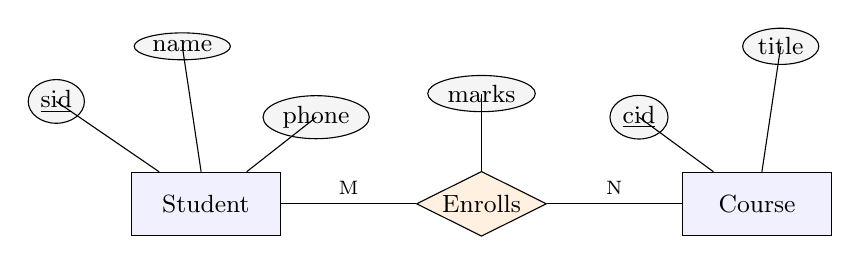
\begin{tikzpicture}[every node/.style={font=\small},node distance=1.2cm,
 ent/.style={draw,rectangle,minimum width=1.9cm,minimum height=0.8cm,fill=blue!6},
 rel/.style={draw,diamond,aspect=2,fill=orange!12,inner sep=1pt},
 att/.style={draw,ellipse,inner sep=1.5pt,fill=gray!8}]
\node[ent] (S) at (0,0) {Student};
\node[ent] (C) at (7,0) {Course};
\node[rel] (E) at (3.5,0) {Enrolls};
\draw (S)--node[above]{\scriptsize M}(E); \draw (E)--node[above]{\scriptsize N}(C);
\node[att] at (-1.9,1.3) {\underline{sid}}; \draw (S)--(-1.9,1.3);
\node[att] at (-0.3,2.0) {name}; \draw (S)--(-0.3,2.0);
\node[att] at (1.4,1.1) {phone}; \draw (S)--(1.4,1.1);
\node[att] at (5.5,1.1) {\underline{cid}}; \draw (C)--(5.5,1.1);
\node[att] at (7.3,2.0) {title}; \draw (C)--(7.3,2.0);
\node[att] at (3.5,1.4) {marks}; \draw (E)--(3.5,1.4);
\end{tikzpicture}
\end{center}
Here \texttt{Student}--\texttt{Course} is $M{:}N$ and the relationship carries its own attribute \texttt{marks}: it belongs to the \emph{pair}, not to either entity alone.

\subsection{Converting an ER diagram to tables}
\begin{formula}[Conversion rules]
\begin{itemize}[noitemsep]
\item \textbf{Strong entity} $\to$ one table; its key becomes the primary key. Composite attributes are flattened to their simple parts.
\item \textbf{Multivalued attribute} $\to$ a separate table $(\text{owner key},\text{value})$.
\item \textbf{Weak entity} $\to$ a table containing the owner's key plus its partial key; primary key is the combination.
\item $\mathbf{1{:}N}$ relationship $\to$ no new table: put the key of the $1$ side as a foreign key in the $N$ side.
\item $\mathbf{1{:}1}$ relationship $\to$ no new table: add a foreign key to either side (better to the side with total participation).
\item $\mathbf{M{:}N}$ relationship $\to$ a \textbf{new table} holding both keys (together the primary key) and the relationship's attributes.
\item \textbf{Specialization} $\to$ either one table per entity (subclass keyed by the superclass key), or one table for the whole hierarchy with a type column.
\end{itemize}
\textbf{Counting shortcut:} number of tables $=$ (entity sets) $+$ ($M{:}N$ relationships) $+$ (multivalued attributes) [for binary relationships].
\end{formula}
\begin{example}[Counting tables]
An ER diagram has entity sets $E_1,E_2,E_3$. $E_1$--$E_2$ is $M{:}N$, $E_2$--$E_3$ is $1{:}N$, $E_1$--$E_3$ is $1{:}1$. Tables: $3$ (entities) $+1$ (the $M{:}N$ relationship) $=\mathbf{4}$; the other two relationships merge into existing tables as foreign keys.
\end{example}
\begin{trap}
(1) A relationship attribute of an $M{:}N$ relationship cannot be moved into either entity. (2) For a $1{:}N$ relationship the foreign key goes on the \emph{many} side. (3) A weak entity has total participation in its identifying relationship. (4) A ternary relationship is not the same as three binary ones.
\end{trap}

% =====================================================================
\section{The Relational Model and Query Languages}

\begin{story}[Registers as tables]
Ramu opens a register: rows are students, columns are facts such as name and department. Somu: ``A \textbf{relation} is exactly such a table. The \textbf{schema} is the column headings (written $\text{Student}(\underline{sid},\text{name},\text{dept},\text{cgpa})$) and the \textbf{instance} is the rows currently in it. Rows are called \textbf{tuples}, columns \textbf{attributes}. The order of rows and of columns does not matter, and there are no duplicate rows in the pure model.''
\end{story}

\subsection{Keys}
\begin{formula}[Kinds of keys]
\begin{itemize}[noitemsep]
\item \textbf{Superkey}: a set of attributes that uniquely identifies every tuple (any superset of a key).
\item \textbf{Candidate key}: a \emph{minimal} superkey (remove any attribute and uniqueness is lost).
\item \textbf{Primary key}: the candidate key chosen for the table; cannot be \texttt{NULL}. The others are \textbf{alternate keys}.
\item \textbf{Foreign key}: attributes in one table that refer to the primary key of another (or the same) table. They may repeat and may be \texttt{NULL} (unless forbidden).
\item \textbf{Prime attribute}: part of at least one candidate key; otherwise \textbf{non-prime}.
\end{itemize}
\end{formula}

\subsection{Relational algebra}
\begin{center}
\small
\begin{tabularx}{\textwidth}{>{\raggedright\arraybackslash}p{3.2cm}>{\raggedright\arraybackslash}p{3.2cm}>{\raggedright\arraybackslash}X}
\toprule
\textbf{Operator} & \textbf{Symbol} & \textbf{Meaning and size}\\
\midrule
Selection & $\sigma_{\theta}(R)$ & rows satisfying $\theta$; $\le|R|$ rows, same columns\\
Projection & $\pi_{A_1,\dots}(R)$ & chosen columns, duplicates removed; $\le|R|$ rows\\
Rename & $\rho_{S(B_1,\dots)}(R)$ & renames relation/attributes\\
Union, Intersection, Difference & $R\cup S,\ R\cap S,\ R-S$ & need \emph{union-compatible} schemas; $|R\cup S|\le|R|+|S|$, $|R-S|\le|R|$\\
Cartesian product & $R\times S$ & every pairing; exactly $|R|\cdot|S|$ rows\\
Natural join & $R\bowtie S$ & product, keep rows equal on the common attributes, drop the duplicate columns\\
Theta/equi-join & $R\bowtie_\theta S$ & product followed by $\sigma_\theta$\\
Outer joins & $\bowtie^{L},\ \bowtie^{R},\ \bowtie^{F}$ (left, right, full) & keep unmatched rows of left, right, or both sides, padded with \texttt{NULL}\\
Division & $R\div S$ & values of $R$'s extra attributes paired with \emph{every} tuple of $S$\\
\bottomrule
\end{tabularx}
\end{center}

\begin{formula}[Useful identities and facts]
\begin{itemize}[noitemsep]
\item Join is a derived operator: $R\bowtie_\theta S=\sigma_\theta(R\times S)$. Division is also derived: $R\div S=\pi_X(R)-\pi_X\bigl((\pi_X(R)\times S)-R\bigr)$.
\item Selection pushes below join: $\sigma_{\theta}(R\bowtie S)=\sigma_\theta(R)\bowtie S$ when $\theta$ uses only $R$'s attributes (optimizers do this).
\item If $R$ has a foreign key to $S$'s key (non-null), then $|R\bowtie S|=|R|$.
\item The \textbf{complete set} of operators is $\{\sigma,\pi,\cup,-,\times,\rho\}$: every other operator can be derived.
\item \texttt{NULL} never equals anything (even \texttt{NULL}), so rows with \texttt{NULL} join attributes do not match in a join.
\end{itemize}
\end{formula}

\begin{example}[Division, and join sizes with NULLs]
Let $E(s,c)=\{(a,1),(a,2),(b,1),(c,1),(c,2),(c,3)\}$ (who took which course) and $C(c)=\{1,2\}$. Then $E\div C=\{a,c\}$: only $a$ and $c$ took \emph{both} courses (student $b$ missed course $2$).\\[4pt]
Let $R(a,b)=\{(1,x),(2,x),(3,y),(4,\text{NULL})\}$ and $S(b,c)=\{(x,10),(x,20),(z,30),(\text{NULL},40)\}$.
\begin{itemize}[noitemsep]
\item $R\bowtie S$: $4$ rows (the two $x$-tuples of $R$ with the two $x$-tuples of $S$).
\item Left outer join: $4+2=6$ (adds $(3,y)$ and $(4,\text{NULL})$ with \texttt{NULL}s). Full outer join: $6+2=8$.
\item $R\times S$: $4\times4=16$.
\end{itemize}
\end{example}

\subsection{Tuple relational calculus (TRC) and domain calculus}
\begin{story}[Describe, don't compute]
Relational algebra says \emph{how}: ``first select, then join, then project''. Calculus only says \emph{what} you want: ``the set of all $t$ such that $t$ is a student and\dots''. SQL is a blend, but its \texttt{SELECT--FROM--WHERE} is closest to this calculus.
\end{story}
\begin{formula}[Tuple calculus]
Form: $\{\,t\mid P(t)\,\}$ where $P$ is a formula built from atoms $R(t)$ (tuple $t$ is in relation $R$), comparisons such as $t.A>s.B$ or $t.A=5$, connectives $\wedge,\vee,\neg$, and quantifiers $\exists s\in R$, $\forall s\in R$.\\
Example, students with a mark above $80$: $\{t\mid \text{Student}(t)\wedge\exists e\,(\text{Enroll}(e)\wedge e.sid=t.sid\wedge e.marks>80)\}$.\\
Example with $\forall$ (division-like): students who took \emph{every} $4$-credit course:
\[\{t\mid \text{Student}(t)\wedge\forall c\,\bigl(\text{Course}(c)\wedge c.credits=4\Rightarrow\exists e\,(\text{Enroll}(e)\wedge e.sid=t.sid\wedge e.cid=c.cid)\bigr)\}\]
A formula is \textbf{safe} if it can only produce finitely many tuples from values in the database; unsafe examples are like $\{t\mid\neg\text{Student}(t)\}$. Safe tuple calculus is exactly as expressive as relational algebra.\\
\textbf{Domain relational calculus} uses \emph{variables over attribute values}: $\{\langle n,d\rangle\mid\exists s\,(\langle s,n,d,g\rangle\in\text{Student}\wedge g>8)\}$ (QBE is based on it).
\end{formula}
\begin{trap}
(1) Relational algebra \emph{removes duplicates}; SQL does not unless told to (\texttt{DISTINCT}). (2) Natural join joins on \emph{all} common attribute names; with no common attribute it becomes a Cartesian product. (3) Union needs the same number and compatible types of columns. (4) $R\div S$ is not simply ``$R-S$''.
\end{trap}
% =====================================================================
\section{SQL}

\begin{story}[Asking the office clerk]
Ramu wants answers from the student register. Somu: ``You do not walk through the files yourself. You write the question in a language the clerk understands and say \emph{what} you want, not \emph{how} to find it. That language is \textbf{SQL}.'' We will use one small college database throughout.
\end{story}

\begin{lstlisting}[style=sql]
CREATE TABLE Student(sid INTEGER PRIMARY KEY, name TEXT NOT NULL,
                     dept TEXT, cgpa REAL CHECK (cgpa BETWEEN 0 AND 10));
CREATE TABLE Course(cid TEXT PRIMARY KEY, title TEXT, credits INTEGER);
CREATE TABLE Enroll(sid INTEGER REFERENCES Student(sid) ON DELETE CASCADE,
                    cid TEXT REFERENCES Course(cid), marks INTEGER,
                    PRIMARY KEY (sid, cid));
\end{lstlisting}
\begin{center}
\small
\begin{tabular}{@{}l@{\hspace{1.2cm}}l@{\hspace{1.2cm}}l@{}}
\begin{tabular}{rlll}
\multicolumn{4}{l}{\textbf{Student}}\\\toprule
sid&name&dept&cgpa\\\midrule
1&Asha&CS&8.5\\2&Ravi&EE&7.0\\3&Meena&CS&9.1\\4&Kiran&ME&6.5\\5&Tara&EE&NULL\\\bottomrule
\end{tabular}&
\begin{tabular}{lll}
\multicolumn{3}{l}{\textbf{Course}}\\\toprule
cid&title&credits\\\midrule
C1&DBMS&4\\C2&Maths&3\\C3&ML&4\\\bottomrule
\end{tabular}&
\begin{tabular}{rlr}
\multicolumn{3}{l}{\textbf{Enroll}}\\\toprule
sid&cid&marks\\\midrule
1&C1&85\\1&C2&78\\2&C1&62\\3&C1&91\\3&C3&88\\4&C2&55\\\bottomrule
\end{tabular}
\end{tabular}
\end{center}

\subsection{Order of evaluation}
\begin{formula}[Logical order in which a SELECT is processed]
\texttt{FROM} (joins) $\to$ \texttt{WHERE} (filter rows) $\to$ \texttt{GROUP BY} $\to$ \texttt{HAVING} (filter groups) $\to$ \texttt{SELECT} (compute columns, aggregates) $\to$ \texttt{DISTINCT} $\to$ \texttt{ORDER BY} $\to$ \texttt{LIMIT}.\\
Hence: \texttt{WHERE} cannot use aggregates, \texttt{HAVING} can; any non-aggregated column in \texttt{SELECT} must appear in \texttt{GROUP BY}.
\end{formula}

\subsection{Selection, joins and aggregation (all outputs real)}
\begin{lstlisting}[style=sql]
SELECT s.name, c.title, e.marks
FROM Student s JOIN Enroll e ON s.sid=e.sid JOIN Course c ON c.cid=e.cid
WHERE e.marks > 80 ORDER BY s.name;
\end{lstlisting}
\begin{lstlisting}[style=out]
(Asha, DBMS, 85)   (Meena, DBMS, 91)   (Meena, ML, 88)
\end{lstlisting}
\begin{lstlisting}[style=sql]
SELECT dept, COUNT(*), COUNT(cgpa), AVG(cgpa) FROM Student GROUP BY dept;
\end{lstlisting}
\begin{lstlisting}[style=out]
(CS, 2, 2, 8.8)   (EE, 2, 1, 7.0)   (ME, 1, 1, 6.5)
\end{lstlisting}
Note the EE row: \texttt{COUNT(*)} $=2$ counts both rows, but \texttt{COUNT(cgpa)} $=1$ and \texttt{AVG}$=7.0$ because aggregates \emph{ignore NULL}.
\begin{lstlisting}[style=sql]
SELECT sid, AVG(marks) FROM Enroll GROUP BY sid HAVING AVG(marks) > 80;
\end{lstlisting}
\begin{lstlisting}[style=out]
(1, 81.5)   (3, 89.5)
\end{lstlisting}

\begin{formula}[Aggregates and NULL]
\texttt{COUNT(*)} counts rows; \texttt{COUNT(col)}, \texttt{SUM}, \texttt{AVG}, \texttt{MIN}, \texttt{MAX} skip \texttt{NULL}s. On an empty set \texttt{COUNT} gives $0$ but \texttt{SUM/AVG/MIN/MAX} give \texttt{NULL}. \texttt{AVG}$=\texttt{SUM}/\texttt{COUNT(col)}$ over non-null values only.
\end{formula}

\subsection{Joins}
\begin{center}
\small
\begin{tabularx}{\textwidth}{>{\raggedright\arraybackslash}p{3.8cm}>{\raggedright\arraybackslash}X}
\toprule
\textbf{Join} & \textbf{Result}\\
\midrule
\texttt{INNER JOIN} / \texttt{JOIN} & only matching pairs\\
\texttt{LEFT [OUTER] JOIN} & all left rows; unmatched ones get \texttt{NULL} on the right\\
\texttt{RIGHT [OUTER] JOIN} & mirror image\\
\texttt{FULL [OUTER] JOIN} & all rows from both sides\\
\texttt{CROSS JOIN} / comma & Cartesian product: $|R|\cdot|S|$ rows (here $5\times3=15$)\\
\texttt{NATURAL JOIN} & equality on all common column names\\
\bottomrule
\end{tabularx}
\end{center}
\begin{lstlisting}[style=sql]
SELECT s.name, COUNT(e.cid) FROM Student s LEFT JOIN Enroll e ON s.sid=e.sid GROUP BY s.sid;
\end{lstlisting}
\begin{lstlisting}[style=out]
(Asha,2) (Ravi,1) (Meena,2) (Kiran,1) (Tara,0)     <- Tara appears with 0
\end{lstlisting}
With an \emph{inner} join the same query drops Tara (she has no enrolment). Counting \texttt{e.cid} (not \texttt{*}) gives $0$ for her; \texttt{COUNT(*)} would wrongly give $1$.

\subsection{Subqueries}
\begin{story}[A question inside a question]
``Who scored above the class average?'' needs the average first. Somu writes it as a \textbf{subquery}: a query in brackets used as a value, a list, or a yes/no test. A \textbf{correlated} subquery refers to the outer row and is re-evaluated for each outer row.
\end{story}
\begin{lstlisting}[style=sql]
-- students above the average cgpa (AVG ignores NULL: (8.5+7+9.1+6.5)/4 = 7.775)
SELECT name FROM Student WHERE cgpa > (SELECT AVG(cgpa) FROM Student);   -- Asha, Meena

-- students enrolled in no course (correlated NOT EXISTS)
SELECT name FROM Student s WHERE NOT EXISTS (SELECT 1 FROM Enroll e WHERE e.sid=s.sid);  -- Tara

-- second highest cgpa
SELECT MAX(cgpa) FROM Student WHERE cgpa < (SELECT MAX(cgpa) FROM Student);   -- 8.5

-- division in SQL: students who took EVERY 4-credit course (double NOT EXISTS)
SELECT name FROM Student s WHERE NOT EXISTS (
  SELECT * FROM Course c WHERE c.credits=4 AND NOT EXISTS (
    SELECT * FROM Enroll e WHERE e.sid=s.sid AND e.cid=c.cid));          -- Meena
\end{lstlisting}
\textbf{Set operations} on the C1 and C2 enrolments: \texttt{INTERSECT} gives $\{1\}$, \texttt{UNION} gives $\{1,2,3,4\}$, \texttt{EXCEPT} (C1 minus C2) gives $\{2,3\}$. Set operators remove duplicates (\texttt{UNION ALL} keeps them).

\subsection{NULL and three-valued logic}
\begin{formula}[NULL rules]
Any comparison with \texttt{NULL} yields \textbf{UNKNOWN}, not true or false. A \texttt{WHERE} keeps only rows where the condition is \textbf{TRUE}. Test with \texttt{IS NULL}. Truth tables: $\text{T}\wedge\text{U}=\text{U}$, $\text{F}\wedge\text{U}=\text{F}$, $\text{T}\vee\text{U}=\text{T}$, $\text{F}\vee\text{U}=\text{U}$, $\neg\text{U}=\text{U}$.
\end{formula}
\begin{lstlisting}[style=sql]
SELECT COUNT(*) FROM Student WHERE cgpa = NULL;                 -- 0   (never true!)
SELECT name FROM Student WHERE cgpa <> 8.5;                      -- Ravi, Meena, Kiran (Tara lost)
SELECT name FROM Student WHERE cgpa <> 8.5 OR cgpa IS NULL;      -- Ravi, Meena, Kiran, Tara
\end{lstlisting}
\begin{trap}
(1) \texttt{x NOT IN (subquery)} returns \emph{nothing at all} if the subquery contains a \texttt{NULL}: with $A=\{1,2,3\}$ and $B=\{1,\text{NULL}\}$, \texttt{SELECT x FROM A WHERE x NOT IN (SELECT y FROM B)} returns an empty result, while the \texttt{NOT EXISTS} version returns $\{2,3\}$. (2) \texttt{WHERE} cannot contain \texttt{COUNT(*)}; use \texttt{HAVING}. (3) \texttt{COUNT(*)} versus \texttt{COUNT(col)} with NULLs. (4) \texttt{ORDER BY} sorts \texttt{NULL}s first or last depending on the system. (5) \texttt{LIKE '\_a\%'}: \texttt{\_} is exactly one character and \texttt{\%} is any string; here it matches Ravi and Tara. (6) \texttt{DISTINCT} applies to the whole selected row, not one column.
\end{trap}

\subsection{Other statements worth knowing}
\begin{lstlisting}[style=sql]
INSERT INTO Course VALUES ('C4','AI',3);
UPDATE Student SET cgpa = cgpa + 0.1 WHERE dept = 'CS';
DELETE FROM Enroll WHERE marks < 40;
ALTER TABLE Student ADD COLUMN email TEXT;
DROP TABLE Enroll;                                   -- removes structure and data
CREATE VIEW TopStudents AS SELECT * FROM Student WHERE cgpa > 8;   -- a stored query
CREATE INDEX idx_dept ON Student(dept);                            -- speeds up lookups
\end{lstlisting}
A \textbf{view} is a virtual table (its definition is stored, not its data). \texttt{DELETE} removes rows (can be rolled back and filtered), \texttt{TRUNCATE} empties a table quickly, \texttt{DROP} removes the table itself.

% =====================================================================
\section{Integrity Constraints}

\begin{story}[The strict librarian]
Somu's librarian refuses to issue a card without a name, refuses two cards with the same number, and refuses to record a loan for a book that is not in the catalogue. ``These rules are \textbf{integrity constraints}: the database itself rejects wrong data, no matter who types it.''
\end{story}

\begin{formula}[Types of constraints]
\begin{itemize}[noitemsep]
\item \textbf{Domain constraint}: values must come from the declared type and satisfy \texttt{CHECK} (e.g.\ $0\le\text{cgpa}\le10$); \texttt{NOT NULL}.
\item \textbf{Key constraint}: \texttt{UNIQUE}/\texttt{PRIMARY KEY} values cannot repeat.
\item \textbf{Entity integrity}: no component of a primary key can be \texttt{NULL}.
\item \textbf{Referential integrity}: every non-null foreign-key value must exist as a primary-key (or unique) value in the referenced table.
\item \textbf{Semantic constraints}: business rules through triggers or assertions.
\end{itemize}
\end{formula}

\begin{formula}[Referential actions when the referenced row is deleted or updated]
\texttt{NO ACTION/RESTRICT}: reject the operation. \texttt{CASCADE}: delete/update the referencing rows too. \texttt{SET NULL}: set the foreign key to \texttt{NULL}. \texttt{SET DEFAULT}: set it to the default.\\
Which operations can violate referential integrity? \textbf{Insert} into the \emph{referencing} (child) table, \textbf{delete} from the \emph{referenced} (parent) table, and \textbf{update} of either key.
\end{formula}

\begin{lstlisting}[style=sql]
INSERT INTO Enroll VALUES (9,'C1',50);        -- student 9 does not exist
INSERT INTO Student VALUES (6,'Zed','CS',11); -- violates CHECK (cgpa BETWEEN 0 AND 10)
INSERT INTO Student VALUES (1,'Dup','CS',5);  -- duplicate primary key
DELETE FROM Course WHERE cid='C1';            -- still referenced by Enroll
DELETE FROM Student WHERE sid=1;              -- ON DELETE CASCADE removes Asha's Enroll rows
\end{lstlisting}
\begin{lstlisting}[style=out]
FOREIGN KEY constraint failed
CHECK constraint failed: cgpa BETWEEN 0 AND 10
UNIQUE constraint failed: Student.sid
FOREIGN KEY constraint failed
(the delete succeeds; the SELECT afterwards finds no Enroll rows for sid 1)
\end{lstlisting}
\begin{trap}
(1) A foreign key may be \texttt{NULL} (``no reference yet''); a primary key may not. (2) \texttt{UNIQUE} allows \texttt{NULL}s (how many depends on the system); \texttt{PRIMARY KEY} does not. (3) Referential integrity only checks that the \emph{value exists}; it says nothing about which row is ``correct''. (4) Deleting a parent row is the dangerous operation, not inserting one.
\end{trap}
% =====================================================================
\section{Functional Dependencies and Normalization}

\begin{story}[The messy register]
Somu keeps one big register with columns \texttt{student, course, teacher, teacher's room}. ``Look at the trouble,'' he says. If a teacher changes rooms, \emph{every} row mentioning her must be edited (an \textbf{update anomaly}). A new teacher with no students yet cannot be recorded (an \textbf{insertion anomaly}). Deleting the last student of a course also deletes the only record of the teacher (a \textbf{deletion anomaly}). ``The cure is to split the register so that each fact is stored \emph{once}: that is \textbf{normalization}.''
\end{story}

\subsection{Functional dependencies and closure}
\begin{formula}[Functional dependency]
$X\to Y$ (``$X$ determines $Y$'') means: any two tuples that agree on $X$ also agree on $Y$. It is a statement about \emph{all legal instances}, a rule of the real world, not something you read off one table. $X$ is a \textbf{superkey} of $R$ iff $X\to R$.\\
\textbf{Trivial} if $Y\subseteq X$. \textbf{Armstrong's axioms:} \emph{reflexivity} ($Y\subseteq X\Rightarrow X\to Y$), \emph{augmentation} ($X\to Y\Rightarrow XZ\to YZ$), \emph{transitivity} ($X\to Y,\,Y\to Z\Rightarrow X\to Z$). They are sound and complete. Derived: \emph{union} ($X\to Y,X\to Z\Rightarrow X\to YZ$), \emph{decomposition} ($X\to YZ\Rightarrow X\to Y$ and $X\to Z$), \emph{pseudo-transitivity} ($X\to Y,\,WY\to Z\Rightarrow WX\to Z$).
\end{formula}
\begin{formula}[Attribute closure $X^{+}$ (the workhorse)]
Start with $X^+=X$. Repeat: if some FD $L\to R$ has $L\subseteq X^+$, add $R$ to $X^+$. Stop when nothing changes. Then $X\to Y$ follows from $F$ iff $Y\subseteq X^+$, and $X$ is a superkey iff $X^+$ contains all attributes.\\
\textbf{Candidate-key shortcuts:} attributes that appear \emph{only} on the left of every FD (or on no FD) must be in every key; attributes that appear only on the right are in no key. Start from the compulsory attributes, compute the closure, and add attributes only if needed.
\end{formula}

\begin{example}[Finding keys: $R(A,B,C,D,E)$ with $F=\{A\to B,\ BC\to E,\ ED\to A\}$]
$C$ and $D$ never appear on a right side, so they are in every key. Try $CD$: $(CD)^+=CD$, not everything. Add one more attribute:
\begin{itemize}[noitemsep]
\item $(ACD)^+$: $A\to B$ gives $ACDB$; $BC\to E$ gives $E$. All of $ABCDE$. \checkmark
\item $(BCD)^+$: $BC\to E$ gives $E$; $ED\to A$ gives $A$. All of $ABCDE$. \checkmark
\item $(CDE)^+$: $ED\to A$ gives $A$; $A\to B$ gives $B$. All of $ABCDE$. \checkmark
\end{itemize}
So the candidate keys are $\{ACD,\ BCD,\ CDE\}$. Every attribute is prime. (Verified by brute force.)
\end{example}

\subsection{Normal forms}
\begin{formula}[1NF, 2NF, 3NF, BCNF]
\begin{itemize}[noitemsep]
\item \textbf{1NF}: every attribute is atomic (no repeating groups or sets in a cell).
\item \textbf{2NF}: 1NF and no \emph{partial dependency}: no non-prime attribute depends on a \emph{proper subset} of a candidate key. (Only matters for composite keys.)
\item \textbf{3NF}: for every non-trivial FD $X\to A$: $X$ is a superkey \textbf{or} $A$ is prime. (Equivalently: no non-prime attribute is transitively dependent on a key.)
\item \textbf{BCNF}: for every non-trivial FD $X\to Y$: $X$ is a superkey. (Stricter: the ``or $A$ is prime'' escape is removed.)
\end{itemize}
\[\text{BCNF}\subset\text{3NF}\subset\text{2NF}\subset\text{1NF}.\]
The mnemonic: \emph{every non-key attribute must depend on ``the key (1NF), the whole key (2NF), and nothing but the key (3NF/BCNF), so help me Codd.''}
\end{formula}

\begin{example}[Identifying the highest normal form, five relations (all checked by program)]
\begin{center}
\small
\begin{tabularx}{\textwidth}{>{\raggedright\arraybackslash}p{4.4cm}>{\raggedright\arraybackslash}p{3.2cm}>{\raggedright\arraybackslash}X}
\toprule
\textbf{Relation and FDs} & \textbf{Candidate keys} & \textbf{Highest form and why}\\
\midrule
$R(A,B,C,D)$; $A\to B,\ C\to D$ & $AC$ & \textbf{1NF}: $B$ depends on part $A$ of the key (partial)\\
$R(A,B,C)$; $A\to B,\ B\to C$ & $A$ & \textbf{2NF}: $C$ depends on $A$ through $B$ (transitive), $B$ not a key\\
$R(S,C,I)$; $SC\to I,\ I\to C$ & $SC,\ SI$ & \textbf{3NF, not BCNF}: $I\to C$ but $I$ is not a superkey; $C$ is prime\\
$R(A,B,C)$; $AB\to C,\ C\to B$ & $AB,\ AC$ & \textbf{3NF, not BCNF}: $C\to B$, $C$ not a superkey, $B$ prime\\
$R(A,B,C,D)$; $A\to B,B\to C,C\to D,D\to A$ & $A,B,C,D$ & \textbf{BCNF}: every determinant is a key\\
\bottomrule
\end{tabularx}
\end{center}
\textbf{Fact:} every relation with only two attributes is in BCNF.
\end{example}

\subsection{Decomposition: lossless join and dependency preservation}
\begin{story}[Splitting without losing information]
When Somu splits a table he wants two things. First, he must be able to rebuild the original by joining the pieces, \emph{no more and no fewer} rows (\textbf{lossless}). Second, the rules ($F$) should still be checkable on the pieces without joining them (\textbf{dependency preserving}).
\end{story}
\begin{formula}[Tests]
\begin{itemize}[noitemsep]
\item \textbf{Lossless (binary):} $R$ splits into $R_1,R_2$ losslessly iff $R_1\cap R_2\to R_1$ or $R_1\cap R_2\to R_2$, i.e.\ the common attributes form a key of one piece. For more than two pieces use the \textbf{chase} (tableau) test.
\item \textbf{Dependency preserving:} the union of FDs that hold within each piece (projections of $F$) implies all of $F$.
\item \textbf{BCNF} decomposition is always lossless but may \emph{lose} dependencies. \textbf{3NF} synthesis (from a canonical cover) is \emph{always} lossless and dependency preserving. Neither normal form removes \emph{all} redundancy caused by multivalued dependencies.
\end{itemize}
\end{formula}
\begin{example}[Checking decompositions of $R(A,B,C)$ (verified by chase)]
\begin{itemize}[noitemsep]
\item With $A\to B$: $\{AB,AC\}$ is \textbf{lossless} (common attribute $A$ is a key of $AB$). $\{AB,BC\}$ is \textbf{lossy} (common attribute $B$ is a key of neither).
\item With $B\to C$: $\{AB,BC\}$ is lossless ($B$ is a key of $BC$).
\item $R(S,C,I)$ with $SC\to I,\ I\to C$: BCNF decomposition gives $\{SI,\ IC\}$ (lossless since $I$ is the key of $IC$) but the dependency $SC\to I$ can no longer be checked inside one table: it is \textbf{not preserved}.
\end{itemize}
\end{example}

\subsection{Canonical (minimal) cover}
\begin{formula}[Computing a canonical cover $F_c$]
(1) Split right sides so each FD has a single attribute on the right. (2) Remove \textbf{extraneous attributes} from left sides: in $XA\to B$, $A$ is extraneous if $B\in X^+$ computed with $F$. (3) Remove \textbf{redundant FDs}: delete $X\to A$ if $A\in X^+$ computed from the remaining FDs. The result is not unique, but all minimal covers have the same closure.
\end{formula}
\begin{example}[$F=\{A\to BC,\ B\to C,\ A\to B,\ AB\to C\}$]
Split: $A\to B,\ A\to C,\ B\to C,\ A\to B,\ AB\to C$. Remove the duplicate $A\to B$. In $AB\to C$, $B$ alone already gives $C$ (via $B\to C$), so it is redundant. $A\to C$ is redundant because $A\to B\to C$. The canonical cover is $\{A\to B,\ B\to C\}$ (verified by program).
\end{example}

\subsection{Counting superkeys, and multivalued dependencies}
\begin{itemize}[noitemsep]
\item If a relation of $n$ attributes has a \emph{single} candidate key of $k$ attributes, it has $2^{\,n-k}$ superkeys. For $R(A,B,C,D)$ with key $A$: $2^3=8$. With two single-attribute keys $A$ and $B$ on four attributes: $8+8-4=12$ superkeys (inclusion--exclusion).
\item \textbf{Multivalued dependency} $X\twoheadrightarrow Y$: for each $X$-value, the set of $Y$-values is independent of the remaining attributes. A relation is in \textbf{4NF} if every non-trivial MVD $X\twoheadrightarrow Y$ has $X$ as a superkey. Classic example: \texttt{(person, phone, hobby)} where phones and hobbies are independent: storing all combinations is redundant; split into \texttt{(person, phone)} and \texttt{(person, hobby)}.
\end{itemize}
\begin{trap}
(1) Closure is computed with \emph{all} FDs, and $X\to Y$ is judged by $Y\subseteq X^+$. (2) 3NF allows $X\to A$ with $A$ prime even if $X$ is not a key; BCNF does not. (3) 2NF violations need a \emph{proper subset of a candidate key} on the left. (4) Check \emph{all} candidate keys when deciding which attributes are prime. (5) BCNF decomposition can lose FDs; 3NF cannot. (6) Lossless does \emph{not} imply dependency preserving, and vice versa. (7) A table with a single-attribute candidate key and no other FDs is automatically 2NF (no partial dependencies are possible).
\end{trap}

% =====================================================================
\section{File Organization and Indexing}

\begin{story}[Finding a book in the library]
Ramu wants one book. Plan A: scan every shelf (a \textbf{heap file}: records in arrival order). Plan B: shelves sorted by title, so he can open the middle and halve the search (an \textbf{ordered file}). Plan C: a formula that tells him the exact shelf from the title (a \textbf{hashed file}). Plan D: a small \textbf{card catalogue} listing the title and shelf number, itself sorted: that is an \textbf{index}. Everything here is measured in \emph{block (disk page) accesses}, because reading a disk block costs far more than anything the CPU does in memory.
\end{story}

\subsection{Blocks and file organizations}
\begin{formula}[Basic calculations]
Block size $B$, record size $R$: \textbf{blocking factor} $bfr=\lfloor B/R\rfloor$ records per block (unspanned records). Number of blocks for $r$ records: $b=\lceil r/bfr\rceil$.
\begin{center}
\small
\begin{tabular}{lccc}
\toprule
\textbf{Organization} & \textbf{Search on key} & \textbf{Insert} & \textbf{Range query}\\
\midrule
Heap (unordered) & $b/2$ average, $b$ worst & $1$ (append) & $b$\\
Sorted (ordered) & $\lceil\log_2b\rceil$ & expensive (shift records) & good\\
Hashed & about $1$ & about $1$ & poor\\
\bottomrule
\end{tabular}
\end{center}
\end{formula}

\subsection{Indexes}
\begin{formula}[Kinds of index]
\begin{itemize}[noitemsep]
\item \textbf{Primary index}: on the \emph{ordering key} field of a sorted file. \textbf{Clustering index}: on an ordering \emph{non-key} field. \textbf{Secondary index}: on a non-ordering field; there can be many, and it must be \textbf{dense}.
\item \textbf{Dense} index: one entry for \emph{every} record. \textbf{Sparse} index: one entry per \emph{block} (only possible if the data file is sorted on that field).
\item A file can have at most \textbf{one} primary or clustering index (it can only be sorted one way) but many secondary indexes.
\item \textbf{Multilevel index}: build an index on the index until the top level fits in one block. Search cost $=$ number of levels $+1$ data block.
\end{itemize}
\end{formula}

\begin{example}[Worked numbers: 30\,000 records of 100 bytes, block 1024 bytes, index entry $=8$ B key $+\,6$ B pointer]
\begin{itemize}[noitemsep]
\item $bfr=\lfloor1024/100\rfloor=10$, so $b=30\,000/10=3000$ blocks. (24 bytes per block are wasted.)
\item Binary search on the data file: $\lceil\log_23000\rceil=\mathbf{12}$ block accesses (since $2^{11}=2048<3000\le4096$).
\item Index entries per block: $\lfloor1024/14\rfloor=73$.
\item \textbf{Sparse primary index}: one entry per data block, $3000$ entries, so $\lceil3000/73\rceil=42$ index blocks; binary search in the index $\lceil\log_242\rceil=6$, plus $1$ data block: \textbf{7} accesses.
\item \textbf{Dense secondary index}: $30\,000$ entries, $\lceil30\,000/73\rceil=411$ index blocks; $\lceil\log_2411\rceil=9$, plus $1$: \textbf{10} accesses.
\item \textbf{Multilevel} on the dense index: level sizes $411\to\lceil411/73\rceil=6\to1$ block, so $3$ index levels $+1$ data block $=\mathbf{4}$ accesses.
\end{itemize}
\end{example}

\subsection{B-trees and B$^{+}$-trees}
\begin{story}[A tree that stays short and fat]
A binary tree of a million keys is $20$ levels deep: $20$ disk reads. Somu widens each node to fill a whole disk block, holding about $70$ keys. Now the same million keys need only $3$ or $4$ levels. ``A \textbf{B$^+$-tree} is a balanced, \emph{wide} search tree designed for disks: all leaves are at the same depth, nodes are at least half full, and inserts split nodes instead of making the tree lopsided.''
\end{story}
\begin{formula}[B$^+$-tree facts]
\begin{itemize}[noitemsep]
\item \textbf{Internal nodes} hold only keys and child pointers (a router). \textbf{All data pointers are in the leaves}, and leaves are linked in a list, so range scans follow the chain. In a B-tree, data pointers can also sit in internal nodes.
\item \textbf{Order $p$} (internal node): up to $p$ child pointers and $p-1$ keys. Choose the largest $p$ with $p\cdot P_{ptr}+(p-1)\cdot K\le B$. Every non-root internal node has at least $\lceil p/2\rceil$ children; the root has at least $2$.
\item Leaf of capacity $p_{leaf}$: largest $p_{leaf}$ with $p_{leaf}(K+P_{rec})+P_{ptr}\le B$ (one extra pointer to the next leaf). Non-root leaves are at least $\lceil p_{leaf}/2\rceil$ full.
\item Search, insert, delete all cost $O(\log_p N)$ block accesses. Height grows only when the root splits.
\end{itemize}
\end{formula}
\begin{example}[Order calculation: $B=1024$, key $K=8$, block pointer $6$, record pointer $7$]
Internal: $6p+8(p-1)\le1024\Rightarrow14p\le1032\Rightarrow p=\mathbf{73}$ (check: $73\cdot6+72\cdot8=1014\le1024$; $p=74$ gives $1028$). Leaf: $15\,p_{leaf}+6\le1024\Rightarrow p_{leaf}=\mathbf{67}$. Minimum fill: $37$ children internally, $34$ entries in a leaf.\\
Maximum records indexed by a tree with $k$ levels (root $=$ level $1$, leaves at level $k$): $73^{k-1}\cdot67$.
\begin{center}
\begin{tabular}{c|ccccc}
levels $k$ & 1 & 2 & 3 & 4 & 5\\\midrule
max records & 67 & 4\,891 & 357\,043 & 26\,064\,139 & 1\,902\,682\,147
\end{tabular}
\end{center}
So $1$ million records need at most $4$ levels, i.e.\ $4$ block reads to find any record (plus one for the data block).
\end{example}

\subsection{Hashing}
\begin{itemize}[noitemsep]
\item \textbf{Static hashing:} $h(K)\bmod M$ chooses one of $M$ buckets (blocks). Collisions beyond one block go to \textbf{overflow chains}. Equality lookups $\approx1$ block access; range queries are not supported.
\item \textbf{Dynamic hashing} (\emph{extendible} and \emph{linear} hashing) lets the file grow without rehashing everything: extendible hashing keeps a \textbf{directory} indexed by the first \emph{global depth} bits of the hash, each bucket has a \emph{local depth}, and a full bucket splits (the directory doubles only when local depth would exceed global depth).
\item Rule of thumb: \textbf{B$^+$-tree} for range and equality; \textbf{hash} for equality only; bitmap indexes for low-cardinality columns in warehouses.
\end{itemize}
\begin{trap}
(1) A sparse index needs a \emph{sorted} data file; a secondary index must be dense. (2) Compute $bfr$ with a floor and $b$ with a ceiling. (3) The number of index entries at the next level equals the number of \emph{blocks} at the level below. (4) In a B$^+$-tree the leaf order differs from the internal order because leaves store record pointers. (5) A binary search over $b$ blocks costs $\lceil\log_2b\rceil$ block accesses. (6) An index speeds up reads but slows down inserts and deletes (the index must be updated too).
\end{trap}
% =====================================================================
\section{Data Types and Data Transformation (Preprocessing)}

\begin{story}[Cleaning the exam sheets]
Before any analysis Somu collects the marks sheets from five colleges. One marks out of 100, another out of 10, some boxes are empty, a few say ``1000''. ``If we feed this straight into a program the answers will be nonsense,'' he says. ``First we \emph{clean} and \emph{transform} the data: put everything on one scale, fill or drop the gaps, shrink the size.'' This is \textbf{data preprocessing}.
\end{story}

\subsection{Types of attributes}
\begin{center}
\small
\begin{tabularx}{\textwidth}{>{\raggedright\arraybackslash}p{2.6cm}>{\raggedright\arraybackslash}p{4.2cm}>{\raggedright\arraybackslash}X}
\toprule
\textbf{Type} & \textbf{What is meaningful} & \textbf{Examples}\\
\midrule
Nominal & equality only (labels) & colour, department, PIN code\\
Ordinal & order, but not differences & grades A$>$B$>$C, ratings 1--5\\
Interval & order and differences; no true zero & temperature in $^\circ$C, calendar year\\
Ratio & order, differences, \emph{ratios}; true zero & height, salary, age, count\\
\bottomrule
\end{tabularx}
\end{center}
Also: \textbf{discrete} (countable) vs \textbf{continuous}; \textbf{binary} attributes (symmetric or asymmetric). Only ratio data allow statements like ``twice as much'' ($40^\circ$C is \emph{not} twice as hot as $20^\circ$C).

\subsection{Missing values and noise}
Handling missing values: ignore the record, fill with a constant, the attribute \textbf{mean/median} (or the class-wise mean), the most likely value (prediction), or flag it with an indicator column. \textbf{Noise/outliers:} smoothing by binning (below), regression, or clustering; a common outlier rule flags values outside $[Q_1-1.5\,\mathrm{IQR},\ Q_3+1.5\,\mathrm{IQR}]$.

\subsection{Normalization (rescaling)}
\begin{story}[Making rupees and kilometres comparable]
A distance method treats ``salary $=50\,000$'' and ``age $=30$'' by raw size, so salary would swamp age. Somu rescales each attribute so no single one dominates.
\end{story}
Data used below (12 prices, verified): $d=\{4,8,9,15,21,21,24,25,26,28,29,34\}$, with $\min=4$, $\max=34$, mean $\mu=20.33$, median $22.5$, population standard deviation $\sigma=8.966$.
\begin{formula}[Normalization methods]
\begin{itemize}[noitemsep]
\item \textbf{Min--max} to $[0,1]$: $v'=\dfrac{v-\min}{\max-\min}$. To a new range $[a,b]$: $v'=a+\dfrac{(v-\min)(b-a)}{\max-\min}$. Preserves the shape, but is sensitive to outliers. For $v=21$: $\frac{21-4}{30}=\mathbf{0.5667}$; for $v=8$: $0.1333$.
\item \textbf{Z-score}: $v'=\dfrac{v-\mu}{\sigma}$ (mean $0$, standard deviation $1$). For $v=21$: $\frac{21-20.33}{8.966}=\mathbf{0.0744}$; $v=4$: $-1.8217$; $v=34$: $1.5243$. (With the sample standard deviation $9.3647$ it would be $0.0712$: read whether the question says population or sample.)
\item \textbf{Decimal scaling}: $v'=\dfrac{v}{10^j}$ with $j$ the smallest integer such that $\max|v'|<1$. Here $\max=34$, so $j=2$: $4\to0.04$, $15\to0.15$.
\end{itemize}
\end{formula}

\subsection{Discretization (binning)}
\begin{formula}[Equal-width and equal-depth bins]
\textbf{Equal-width} (equal interval): width $w=\frac{\max-\min}{k}$. For $k=3$: $w=10$, bins $[4,14)$, $[14,24)$, $[24,34]$:
\[\{4,8,9\},\ \{15,21,21\},\ \{24,25,26,28,29,34\}\quad(\text{sizes }3,3,6:\text{ uneven}).\]
\textbf{Equal-depth} (equal frequency): each bin has the same number of values, here $4$:
\[\{4,8,9,15\},\ \{21,21,24,25\},\ \{26,28,29,34\}.\]
\textbf{Smoothing by bin means:} replace by the bin mean: $9,\ 22.75,\ 29.25$ (each value in the bin becomes that number).\\
\textbf{Smoothing by bin boundaries:} replace each value by the nearer of the bin's min and max: $\{4,4,4,15\},\ \{21,21,25,25\},\ \{26,26,26,34\}$.\\
\textbf{Smoothing by bin medians:} $8.5,\ 22.5,\ 28.5$.
\end{formula}
Other discretization: concept hierarchies (age $\to$ young/middle/old), clustering, entropy-based (supervised) splitting.

\subsection{Sampling}
\begin{itemize}[noitemsep]
\item \textbf{Simple random sample without replacement} (SRSWOR): each record has probability $\frac nN$ of being chosen. With $N=10$, $n=3$: $0.3$.
\item \textbf{With replacement} (SRSWR): a record can appear twice. Probability that a specific record appears at least once in $n=3$ draws from $10$: $1-0.9^3=0.271$.
\item \textbf{Stratified sampling}: divide the data into groups (strata, e.g.\ by class) and sample from each, so rare groups are represented.
\item \textbf{Systematic sampling}: every $k$-th record after a random start. \textbf{Cluster sampling}: pick whole groups at random.
\item \textbf{Reservoir sampling}: choose $n$ records uniformly from a stream of unknown length in one pass.
\end{itemize}

\subsection{Compression and data reduction}
\begin{formula}[Compression]
\textbf{Lossless} compression recovers the data exactly (run-length encoding, Huffman coding, dictionary methods such as LZW); \textbf{lossy} compression does not (JPEG, wavelet transforms, PCA-style projection). Data reduction also includes \textbf{dimensionality reduction} (PCA, feature selection), \textbf{numerosity reduction} (sampling, histograms, clustering) and \textbf{aggregation} (data cubes).
\begin{itemize}[noitemsep]
\item \textbf{Run-length encoding}: \texttt{WWWWBBBWW} $\to$ \texttt{4W3B2W} ($9$ symbols to $6$). It helps only when there are long runs.
\item \textbf{Huffman coding}: frequent symbols get short codes; no code is a prefix of another. Frequencies $a{:}45,\ b{:}13,\ c{:}12,\ d{:}16,\ e{:}9,\ f{:}5$ (per 100 symbols) give code lengths $a=1,\ b=c=d=3,\ e=f=4$ and total cost $45\cdot1+13\cdot3+12\cdot3+16\cdot3+9\cdot4+5\cdot4=\mathbf{224}$ bits, versus $\mathbf{300}$ bits for a fixed $3$-bit code. Construction: repeatedly merge the two smallest weights (here $5+9=14$, $12+13=25$, $14+16=30$, $25+30=55$, $45+55=100$).
\end{itemize}
\end{formula}
\begin{trap}
(1) Min--max is \emph{not} the same as z-score; z-scores can be negative and exceed $1$. (2) Equal-width bins can be very unevenly filled; equal-depth bins hold equal counts but have unequal widths. (3) Check the interval endpoints: $[4,14)$ includes $4$ but not $14$. (4) Fit the scaling parameters on training data, then apply them unchanged to test data. (5) Lossy compression is irreversible. (6) Temperature in $^\circ$C is interval data, not ratio.
\end{trap}

% =====================================================================
\section{Data Warehouse Modelling}

\begin{story}[The shop's yearly review]
Ramu runs a chain of shops. The cashier's database (\textbf{OLTP}) records each sale quickly and correctly: ``one pen sold at 10:42''. At year-end the owner asks: ``Total sales by region, by quarter, by product category, compared with last year.'' Running such a huge question on the live billing system would slow the counters. Somu says: ``Copy the history into a separate store built for \emph{questions}, not for transactions. That is a \textbf{data warehouse}.''
\end{story}

\begin{formula}[Definition (Inmon)]
A data warehouse is \textbf{subject-oriented} (organised around subjects such as sales, not applications), \textbf{integrated} (data from many sources made consistent), \textbf{time-variant} (keeps history), and \textbf{non-volatile} (data is loaded and read, not updated in place).
\end{formula}
\begin{center}
\small
\begin{tabularx}{\textwidth}{>{\raggedright\arraybackslash}p{3cm}>{\raggedright\arraybackslash}X>{\raggedright\arraybackslash}X}
\toprule
 & \textbf{OLTP (operational)} & \textbf{OLAP (warehouse)}\\
\midrule
Purpose & day-to-day transactions & analysis, decision support\\
Data & current, detailed, normalised & historical, summarised, denormalised\\
Operations & many short inserts/updates & complex read-mostly queries\\
Users & clerks, many & analysts, few\\
Size & MB--GB & GB--TB+\\
Design & ER/normalised & star/snowflake\\
\bottomrule
\end{tabularx}
\end{center}

\subsection{Multidimensional model: facts, dimensions, measures}
\begin{formula}[Concepts]
\begin{itemize}[noitemsep]
\item \textbf{Fact table}: one row per business event at a chosen \textbf{granularity} (e.g.\ one product sold on one day in one shop). Columns: foreign keys to every dimension plus numeric \textbf{measures} (quantity, amount). It is the biggest table.
\item \textbf{Dimension table}: descriptive context (Date, Product, Store, Customer). Wide, relatively small, denormalised; keyed by a \textbf{surrogate key}.
\item \textbf{Hierarchy} within a dimension: Date: day $\to$ month $\to$ quarter $\to$ year; Location: street $\to$ city $\to$ state $\to$ country. Hierarchies make \emph{roll-up} and \emph{drill-down} possible.
\item \textbf{Measure types} (by how they aggregate): \textbf{distributive} (can be computed from partial aggregates of partitions: \texttt{SUM, COUNT, MIN, MAX}); \textbf{algebraic} (computed from a fixed number of distributive ones: \texttt{AVG}$=\texttt{SUM}/\texttt{COUNT}$, standard deviation); \textbf{holistic} (no constant-size partial summary: \texttt{MEDIAN, MODE, RANK}).
\item \textbf{Additive} measures (amount) can be summed across all dimensions; \textbf{semi-additive} (account balance) cannot be summed across time; \textbf{non-additive} (ratios, percentages) cannot be summed at all.
\end{itemize}
\end{formula}

\subsection{Schemas}
\begin{center}
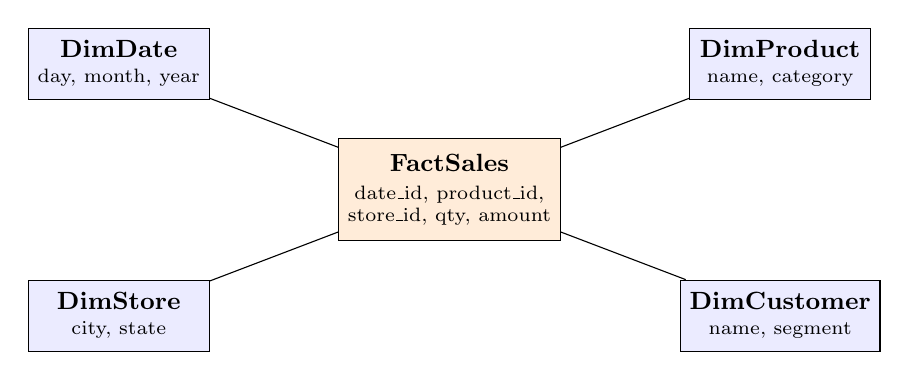
\begin{tikzpicture}[font=\small,
 fact/.style={draw,rectangle,fill=orange!15,minimum width=2.6cm,minimum height=1.3cm,align=center},
 dim/.style={draw,rectangle,fill=blue!8,minimum width=2.3cm,minimum height=0.9cm,align=center}]
\node[fact] (F) at (0,0) {\textbf{FactSales}\\[-1pt]{\scriptsize date\_id, product\_id,}\\[-3pt]{\scriptsize store\_id, qty, amount}};
\node[dim] (D) at (-4.2,1.6) {\textbf{DimDate}\\[-2pt]{\scriptsize day, month, year}};
\node[dim] (P) at (4.2,1.6) {\textbf{DimProduct}\\[-2pt]{\scriptsize name, category}};
\node[dim] (S) at (-4.2,-1.6) {\textbf{DimStore}\\[-2pt]{\scriptsize city, state}};
\node[dim] (C) at (4.2,-1.6) {\textbf{DimCustomer}\\[-2pt]{\scriptsize name, segment}};
\draw (F)--(D); \draw (F)--(P); \draw (F)--(S); \draw (F)--(C);
\end{tikzpicture}
\end{center}
\begin{formula}[Star, snowflake and fact constellation]
\begin{itemize}[noitemsep]
\item \textbf{Star schema} (above): one central fact table directly joined to \emph{denormalised} dimension tables. Fewest joins, fastest queries, some redundancy in dimensions.
\item \textbf{Snowflake schema}: the dimensions are \emph{normalised} into sub-tables (DimProduct $\to$ DimCategory). Less redundancy and storage, but more joins and slower queries.
\item \textbf{Fact constellation (galaxy)}: several fact tables (Sales, Shipping) sharing dimension tables.
\item A \textbf{data mart} is a department-level subset of a warehouse (single subject).
\end{itemize}
\end{formula}

\subsection{OLAP operations (tested on a real star schema)}
\begin{story}[Turning the cube]
Somu pictures sales as a cube whose three edges are \emph{time}, \emph{product} and \emph{place}. Each small cell holds a total. Looking at the cube from different sides is OLAP.
\end{story}
We loaded a tiny warehouse: DimDate ($4$ rows: Jan/Feb of 2025 and 2026), DimProduct ($3$: Pen, Book (Stationery), Mug (Kitchen)), FactSales ($7$ rows; total amount $1080$).
\begin{center}
\small
\begin{tabularx}{\textwidth}{>{\raggedright\arraybackslash}p{3cm}>{\raggedright\arraybackslash}p{4.2cm}>{\raggedright\arraybackslash}X}
\toprule
\textbf{Operation} & \textbf{Meaning} & \textbf{Example result}\\
\midrule
\textbf{Roll-up} & climb a hierarchy or drop a dimension (less detail) & sales by month $\to$ by year: $2025{:}\,410$, $2026{:}\,670$\\
\textbf{Drill-down} & the reverse: more detail & year $\to$ (year, category): $2025$ Kitchen $60$, Stationery $350$; $2026$ Kitchen $120$, Stationery $550$\\
\textbf{Slice} & fix \emph{one} dimension to one value & year $=2025$: Kitchen $60$, Stationery $350$\\
\textbf{Dice} & select values on \emph{two or more} dimensions (a sub-cube) & year $=2026$ and category in $\{\text{Kitchen}\}$\\
\textbf{Pivot (rotate)} & swap rows and columns of the view & categories as columns instead of rows\\
\bottomrule
\end{tabularx}
\end{center}
\begin{lstlisting}[style=sql]
-- roll-up: total sales per year
SELECT year, SUM(amount) FROM FactSales f JOIN DimDate d ON f.d=d.d GROUP BY year;
-- drill-down: add category
SELECT year, category, SUM(amount)
FROM FactSales f JOIN DimDate d ON f.d=d.d JOIN DimProduct p ON f.p=p.p
GROUP BY year, category;
-- slice: year = 2025
... WHERE year = 2025 GROUP BY category;
\end{lstlisting}
\begin{lstlisting}[style=out]
(2025, 410) (2026, 670)
(2025, Kitchen, 60) (2025, Stationery, 350) (2026, Kitchen, 120) (2026, Stationery, 550)
(Kitchen, 60) (Stationery, 350)
\end{lstlisting}

\subsection{The data cube and its lattice}
\begin{formula}[Counting cuboids]
For $n$ dimensions \emph{without hierarchies}, the \textbf{cube} (CUBE operator) contains $\mathbf{2^n}$ \textbf{cuboids}: one for every subset of dimensions to group by. The $n$-dimensional cuboid is the \textbf{base cuboid}; the $0$-dimensional one is the \textbf{apex} (grand total). Examples: $n=3\to8$, $n=4\to16$, $n=10\to1024$.\\
With hierarchies, if dimension $i$ has $L_i$ levels (not counting the virtual level ``all''), the number of cuboids is $\displaystyle\prod_{i=1}^{n}(L_i+1)$. Time (day, month, year) $\to4$, location (city, state, country) $\to4$, product (item, category) $\to3$ gives $4\cdot4\cdot3=\mathbf{48}$.\\
Maximum number of cells in the base cuboid $=\prod|\text{dimension}_i|$: dimensions of sizes $10,5,4$ give $200$ cells. Real cubes are \emph{sparse}: most cells are empty.
\end{formula}

\subsection{ETL, slowly changing dimensions and speed-ups}
\begin{itemize}[noitemsep]
\item \textbf{ETL}: \textbf{E}xtract from sources, \textbf{T}ransform (clean, convert types, rescale, deduplicate, apply business rules), \textbf{L}oad into the warehouse. The preprocessing of the previous section lives in the transform step.
\item \textbf{Slowly changing dimensions} (a customer moves city): \textbf{Type 1} overwrite (history lost); \textbf{Type 2} add a new row with a new surrogate key and validity dates (full history); \textbf{Type 3} add a column for the previous value (limited history).
\item \textbf{Materialised views} and pre-computed cuboids trade storage for speed; \textbf{bitmap indexes} (one bit-vector per distinct value) are ideal for low-cardinality columns such as gender or category, because \texttt{AND/OR} of bitmaps is fast.
\item Warehouse approaches: \textbf{ROLAP} (relational tables), \textbf{MOLAP} (array-based multidimensional storage), \textbf{HOLAP} (hybrid).
\end{itemize}
\begin{trap}
(1) Snowflake normalises the \emph{dimensions}, not the fact table. (2) Slice fixes one dimension; dice restricts several. (3) Roll-up goes \emph{up} the hierarchy (fewer details) \emph{or} removes a dimension. (4) The number of cuboids is $2^n$ only without hierarchies. (5) Median is \emph{holistic}; average is \emph{algebraic}, not distributive. (6) A fact table row must be at one consistent granularity. (7) Warehouse data are mostly loaded and read, not updated.
\end{trap}
% =====================================================================
\section{One-page Cheat Sheet}
\begin{formula}[ER, relational model, algebra]
Tables $=$ entity sets $+$ $M{:}N$ relationships $+$ multivalued attributes. $1{:}N$: foreign key on the $N$ side. Weak entity key $=$ owner key $+$ partial key. $|R\times S|=|R||S|$; $R\bowtie S$ with an FK to $S$'s key has $|R|$ rows. $\{\sigma,\pi,\cup,-,\times,\rho\}$ is a complete set. Division $=$ ``for all''.
\end{formula}
\begin{formula}[SQL]
Order: FROM $\to$ WHERE $\to$ GROUP BY $\to$ HAVING $\to$ SELECT $\to$ ORDER BY. Aggregates skip NULL; \texttt{COUNT(*)} does not. Comparison with NULL is UNKNOWN; use \texttt{IS NULL}. \texttt{NOT IN} with a NULL in the list returns nothing. ``For all'' $=$ double \texttt{NOT EXISTS}. Left join keeps unmatched left rows.
\end{formula}
\begin{formula}[Integrity and normalization]
Keys: superkey $\supset$ candidate (minimal) $\supset$ primary. FK may be NULL; PK may not. Closure $X^+$ decides everything. 2NF: no partial dependency. 3NF: $X$ superkey or $A$ prime. BCNF: $X$ superkey. BCNF$\subset$3NF$\subset$2NF$\subset$1NF. Lossless (binary): common attributes form a key of a piece. BCNF may lose dependencies; 3NF never. Single key of $k$ attributes in $n$: $2^{n-k}$ superkeys.
\end{formula}
\begin{formula}[Files and indexes]
$bfr=\lfloor B/R\rfloor$, $b=\lceil r/bfr\rceil$. Binary search $\lceil\log_2b\rceil$. Sparse index: one entry per block (sorted file). Dense: one per record (secondary). B$^+$-tree: data in leaves, order $p$ from $p\,P+(p-1)K\le B$, height $\approx\log_pN$.
\end{formula}
\begin{formula}[Preprocessing and warehouse]
Min--max $\frac{v-\min}{\max-\min}$; z-score $\frac{v-\mu}{\sigma}$; decimal scaling $v/10^j$. Equal-width vs equal-depth bins. Huffman: merge two smallest. Star: denormalised dimensions; snowflake: normalised. Roll-up/drill-down/slice/dice/pivot. Cuboids: $2^n$ (no hierarchies), $\prod(L_i+1)$ (with). Distributive: sum, count, min, max. Algebraic: avg. Holistic: median.
\end{formula}

% =====================================================================
\section{Practice Questions (with answers)}
Try each one yourself first. Numeric and SQL answers were checked by running code.
\begin{enumerate}[leftmargin=*,itemsep=4pt]
\item An ER diagram has entities $E_1,E_2,E_3$; $E_1$--$E_2$ is $M{:}N$, $E_2$--$E_3$ is $1{:}N$, $E_1$--$E_3$ is $1{:}1$. Minimum number of tables? \textbf{Answer: $4$.}
\item $R(A,B,C,D)$ has the single candidate key $A$. Number of superkeys? \textbf{Answer: $2^3=8$.}
\item $R(A,B,C,D,E)$, $F=\{A\to B,\ BC\to E,\ ED\to A\}$. Candidate keys and highest normal form? \textbf{Answer: $ACD,\ BCD,\ CDE$; 3NF (all attributes prime), not BCNF.}
\item $R(S,C,I)$ with $SC\to I,\ I\to C$. Highest normal form? \textbf{Answer: 3NF, not BCNF} ($I\to C$ with $I$ not a superkey).
\item $R(A,B,C)$, $F=\{A\to B\}$. Is $\{AB,BC\}$ a lossless decomposition? \textbf{Answer: No} (common attribute $B$ is a key of neither piece).
\item Canonical cover of $\{A\to BC,\ B\to C,\ A\to B,\ AB\to C\}$? \textbf{Answer: $\{A\to B,\ B\to C\}$.}
\item $R(A,B,C,D)$ with $A\to B,\ C\to D$. Highest normal form? \textbf{Answer: 1NF} (key $AC$; $B$ and $D$ depend on parts of it).
\item $|R|=1000$, $|S|=500$. Number of tuples in $R\times S$? \textbf{Answer: $500\,000$.}
\item With $R=\{(1,x),(2,x),(3,y),(4,\text{NULL})\}$ and $S=\{(x,10),(x,20),(z,30),(\text{NULL},40)\}$: rows in $R\bowtie S$, left outer join, full outer join? \textbf{Answer: $4,\ 6,\ 8$.}
\item $E=\{(a,1),(a,2),(b,1),(c,1),(c,2),(c,3)\}$, $C=\{1,2\}$. What is $E\div C$? \textbf{Answer: $\{a,c\}$.}
\item On the college database, what does \texttt{SELECT COUNT(*) FROM Student WHERE cgpa = NULL} return? \textbf{Answer: $0$.}
\item Same database, grouping by \texttt{dept} with \texttt{COUNT(*)}, \texttt{COUNT(cgpa)} and \texttt{AVG(cgpa)}: what is the EE row? \textbf{Answer: $(EE,2,1,7.0)$.}
\item Names of students with cgpa above the average cgpa? \textbf{Answer: Asha and Meena} (average $7.775$).
\item \texttt{SELECT x FROM A WHERE x NOT IN (SELECT y FROM B)} with $A=\{1,2,3\}$, $B=\{1,\text{NULL}\}$. \textbf{Answer: empty result.}
\item Number of rows from \texttt{SELECT * FROM Student, Course} ($5$ and $3$ rows)? \textbf{Answer: $15$.}
\item Student LEFT JOIN Enroll, \texttt{COUNT(e.cid)} per student: what does Tara get? \textbf{Answer: $0$} (she appears, with no matches).
\item A referencing-table insert of an Enroll row with a non-existent \texttt{sid}: result? \textbf{Answer: rejected} (referential integrity violation).
\item $30\,000$ records of $100$ B, block $1024$ B: blocking factor and blocks? \textbf{Answer: $10$ and $3000$.}
\item Worst-case block accesses of binary search on those $3000$ blocks? \textbf{Answer: $12$.}
\item Sparse primary index with $14$-byte entries on the same file: total block accesses for a key search? \textbf{Answer: $7$} ($6$ for the $42$-block index $+1$).
\item B$^+$-tree internal order for $B=1024$, key $8$, block pointer $6$? \textbf{Answer: $p=73$.}
\item Min--max value of $21$ in $\{4,8,\dots,34\}$ (min $4$, max $34$)? \textbf{Answer: $0.5667$.}
\item Z-score of $21$ (mean $20.33$, population $\sigma=8.966$)? \textbf{Answer: $0.0744$.}
\item Equal-depth smoothing by bin means of $\{4,8,9,15\}$? \textbf{Answer: every value becomes $9$.}
\item Huffman cost of frequencies $45,13,12,16,9,5$ versus fixed-length? \textbf{Answer: $224$ vs $300$ bits.}
\item Number of cuboids in a 3-dimensional cube; with hierarchies $4,4,3$ levels-plus-all? \textbf{Answer: $8$; $48$.}
\item Which of \texttt{SUM}, \texttt{AVG}, \texttt{MEDIAN} are holistic? \textbf{Answer: only \texttt{MEDIAN}.}
\item In the tiny warehouse, yearly totals after roll-up? \textbf{Answer: $2025{:}\,410$, $2026{:}\,670$.}
\item Which schema normalises its dimensions: star or snowflake? \textbf{Answer: snowflake.}
\end{enumerate}

\textbf{How to study this section:} Spend most of your time on SQL (writing and tracing queries, NULL behaviour, joins, \texttt{GROUP BY/HAVING}, subqueries), normalization (closure, candidate keys, normal-form identification, decomposition tests), and the numeric file/index calculations. Then relational algebra and tuple calculus, preprocessing formulas, and warehouse vocabulary (star vs snowflake, OLAP operations, cuboid counts). Hand-solve $10$ questions on keys and normal forms and $10$ on SQL output, and keep an error log.

\end{document}
